\documentclass{beamer}
\usepackage[utf8]{inputenc}
\usepackage[english]{babel}
\usepackage{graphicx}
\usepackage{booktabs}
\usepackage{multicol}
\usepackage{amsmath}
\usepackage{hyperref}
\usepackage{changes}
\usepackage{url}

\usetheme{Madrid}

\title{Financial Networks Stability Under Technological Uncertainty}
\author{Sebastián Cea \\ Hernán Venegas}
\date{June 27, 2025 \\ Universidad de Los Andes}

\begin{document}

\frame{\titlepage}

\begin{frame}{Background: Alternative vs Traditional Systems}
\begin{itemize}
    \item \textbf{Traditional Systems:}
    \begin{itemize}
        \item Offer \textcolor{blue}{stability and institutional trust} backed by regulatory frameworks.
        \item High costs due to intermediation (banks, brokers).
    \end{itemize}
    
    \item \textbf{Technological Revolution:}
    \begin{itemize}
        \item Blockchain emerges in 1991, Bitcoin in 2008, and decentralized finance (DeFi) concept in 2017.
    \end{itemize}
    
    \item \textbf{Blockchain:}
    \begin{itemize}
        \item Offers \textcolor{blue}{direct transactions without intermediaries}, with greater transparency and traceability, and \textcolor{blue}{lower costs}.
        \item However, presents security risks, volatility, and potential slowness.
    \end{itemize}
\end{itemize}
\end{frame}


\begin{frame}{Background: Global Impact}
\begin{itemize}
    \item \textbf{Economic Potential:}
    \begin{itemize}
        \item Blockchain technologies could \textcolor{red}{boost the global economy by US\$1.76 trillion} by 2030 by increasing levels of tracking, tracing, and trust according to PWC \cite{pwc2020}.
        \item The global Blockchain FinTech market was estimated at US\$3.4 billion in 2024 and is \textcolor{red}{projected to reach US\$49.2 billion by 2030}, growing at a CAGR of 55.9\% between those years  \cite{market_research_future2024}.
    \end{itemize}
\end{itemize}
\end{frame}

\begin{frame}{Motivation}
\begin{itemize}
   \item \textbf{Blockchain is changing the financial world:}
   \begin{itemize}
       \item Opened the door to a \textcolor{blue}{system without intermediaries}, borderless and with a promise of total transparency.
       \item But with \textcolor{red}{risks of hacks, vulnerabilities, volatility} and the uncertainty of an \textcolor{red}{unregulated environment}.
   \end{itemize}
   
   \vspace{0.5cm}
   \item \textbf{Critical questions:}
   \begin{itemize}
  \item How should financial agents \textcolor{blue}{choose} between these two systems?
     \vspace{0.3cm}
   \item Will blockchain replace the traditional system or coexist in equilibrium?
   
   \vspace{0.3cm}
   
   \item What economic characteristics will \textcolor{blue}{determine the adoption} of these technologies?
   \end{itemize}
\end{itemize}
\end{frame}

\begin{frame}{Research Questions}
\textbf{Key questions we address:}
\begin{enumerate}
    \item Under what conditions do agents \textcolor{blue}{adopt blockchain} over traditional systems?
    \item How do \textcolor{red}{transparency benefits} ($\tau$) affect network formation?
    \item What role do \textcolor{red}{transaction frictions} ($\lambda_B$) play in adoption?
    \item When do we observe \textcolor{blue}{coexistence} vs. \textcolor{blue}{dominance} of one network?
\end{enumerate}

\vspace{0.3cm}
\textbf{Our approach:} Extend Jalan et al. (2024) to model competing networks with different technological characteristics.
\end{frame}

\begin{frame}{Why This Base Model?}
\textbf{Objective:} Study endogenously the formation of a transfer network and the impact of a competing network emergence.

\vspace{0.5cm}
\textbf{Why Jalan et al. (2024)?}
\begin{itemize}
    \item Allows modeling the \textcolor{blue}{endogenous formation} of financial networks
    \item Captures \textcolor{blue}{utility maximization} behavior of heterogeneous agents
    \item Incorporates \textcolor{blue}{subjective beliefs} and differentiated risk aversion
    \item Provides existence and \textcolor{blue}{uniqueness conditions} for equilibrium
\end{itemize}

\vspace{0.3cm}
\textbf{Our contribution:} We extend the model to include a second network (blockchain) that competes with the traditional network in transparency and cost dimensions.
\end{frame}

\begin{frame}{Base Model: Network Structure}
\textbf{Network representation:} $n$ agents connected by a weighted network $W\in\mathbb{R}^{n\times n}$

\vspace{0.3cm}
\textbf{Contract structure:}
\begin{itemize}
    \item \textbf{Contract sizes:} $W_{ij}$ = size of contract between agents $i$ and $j$
    \begin{itemize}
        \item Symmetric: $W_{ij} = W_{ji}$ (mutual agreement required)
        \item Can be positive, negative, or zero
    \end{itemize}
    
    \item \textbf{Contract pricing:} $P_{ji} = -P_{ij}$ (zero-sum payments)
    \begin{itemize}
        \item Transaction amount: $P_{ji} \cdot W_{ji}$
        \item Allows side payments for agreement
    \end{itemize}
\end{itemize}

\vspace{0.3cm}
\textbf{Key feature:} Contracts emerge endogenously from agent interactions, not imposed exogenously.
\end{frame}

\begin{frame}{Agent Characteristics and Beliefs}
\textbf{Each agent $i$ is characterized by:}

\begin{itemize}
    \item \textbf{Subjective beliefs:} $\mu_i \in \mathbb{R}^n$
    \begin{itemize}
        \item Expected profitability from contracts with each agent
        \item Can differ across agents (heterogeneous beliefs)
    \end{itemize}
    
    \item \textbf{Risk perception:} $\Sigma_i \succ 0$
    \begin{itemize}
        \item Covariance matrix of perceived risks
        \item Captures correlations between different contracts
    \end{itemize}
    
    \item \textbf{Risk preferences:} $\gamma_i > 0$
    \begin{itemize}
        \item Risk aversion parameter
        \item Higher $\gamma_i$ → more conservative agent
    \end{itemize}
    
    \item \textbf{Constraints:} $\Psi_i$
    \begin{itemize}
        \item Regulatory or operational limitations
        \item Determines feasible contract set
    \end{itemize}
\end{itemize}
\end{frame}

\begin{frame}{Agent Behavior: Utility Maximization}
\textbf{Mean-variance utility function:}
\begin{equation}
g_i(W,P) = w_i^\top (\mu_i - P e_i) - \gamma_i \cdot w_i^\top \Sigma_i w_i
\end{equation}

\vspace{0.3cm}
\textbf{Economic interpretation:}
\begin{itemize}
    \item \textbf{Expected return:} $w_i^\top (\mu_i - P e_i)$
    \begin{itemize}
        \item $w_i$: agent $i$'s portfolio vector
        \item $\mu_i - P e_i$: net expected returns after prices
    \end{itemize}
    
    \item \textbf{Risk penalty:} $\gamma_i \cdot w_i^\top \Sigma_i w_i$
    \begin{itemize}
        \item Higher $\gamma_i$ → more risk-averse agent
        \item $\Sigma_i$: agent $i$'s perceived risk structure
    \end{itemize}
\end{itemize}

\vspace{0.3cm}
\textbf{Optimization:} Each agent chooses portfolio to maximize utility subject to constraints $\Psi_i$.
\end{frame}

\begin{frame}{Equilibrium: Stable Network Formation}
\textbf{Optimal portfolio solution:}
$$w_i^* = Q_i(\mu_i - Pe_i)$$
where: $Q_i = \Psi_i^\top(2\gamma_i\Psi_i\Sigma_i\Psi_i^\top)^{-1}\Psi_i$

\vspace{0.3cm}
\textbf{Equilibrium conditions:}
\begin{itemize}
    \item \textbf{Feasibility:} $W = W^T$, $P = -P^T$, constraints satisfied
    \item \textbf{Stability:} Each agent maximizes utility given prices $P$
    \item \textbf{Market clearing:} All agents agree on contract sizes
\end{itemize}

\end{frame}

\begin{frame}{Original Example 5}
 \vspace{-0.3cm}
 
   \footnotesize
   \begin{itemize}
     \item {Three agents:} National Bank, Local Bank, and Local Firm, but the Local Firm cannot access National Bank directly.
     \item Starting from zero contracts, firms negotiate iteratively.
     \item In $\sim$10 iterations, stable equilibrium is reached.
     \item Local Bank becomes crucial intermediary for indirect capital flows.
   \end{itemize}

 \centering
 
\includegraphics[width=0.9\textwidth,height=0.3\textheight,keepaspectratio]{docs/Diapos/W_original.png}


\includegraphics[width=0.9\textwidth,height=0.3\textheight,keepaspectratio]{docs/Diapos/P_original.png}
 
\end{frame}

\begin{frame}{Original Example 5}
 \vspace{-0.3cm}
 
   \footnotesize
   \begin{itemize}
     \item When there are no restrictions this is the stable network.
     \item This is the stable network that we use as benchmark $w^*$, an ideal scenario without restrictions.
   \end{itemize}

 \centering

\includegraphics[width=0.9\textwidth,height=0.3\textheight,keepaspectratio]{docs/Diapos/W_original_SR.png}


\includegraphics[width=0.9\textwidth,height=0.3\textheight,keepaspectratio]{docs/Diapos/P_original_SR.png}
\end{frame}


\begin{frame}{Model Extension: Dual Network Structure}
Now we extend the model to a secon network (blockchain).
\textbf{New setup:} Agents can choose between two networks

Network configuration: $(\mu_i, \gamma_i, \Sigma_i, \Psi_i^T, \Psi_i^B, \tau, \lambda_B)_{i \in [n]}$

\vspace{0.3cm}
\textbf{New parameters:}
\begin{itemize}
   \item $\Psi_i^T \in \{0,1\}^{|J_i^T| \times n}$: constraints in traditional network
   \item $\Psi_i^B \in \{0,1\}^{|J_i^B| \times n}$: constraints in blockchain network
   \item $\tau \in \mathbb{R}$: \textcolor{blue}{transparency benefit} in blockchain
   \item $\lambda_B \in \mathbb{R}$: \textcolor{red}{friction cost} in blockchain
\end{itemize}

\vspace{0.3cm}
\textbf{Key insight:} Agents optimally allocate between networks based on relative benefits and costs.
\end{frame}

\begin{frame}{Extended Utility Functions}
\textbf{Total utility:} 
$$g_i(w_i^T,w_i^B, P) = g_i^T(w_i^T,P) + g_i^B(w_i^B,P)$$

\vspace{0.3cm}
\textbf{Network-specific utilities:}
\begin{itemize}
    \item \textbf{Traditional:} $g_i^T(w_i^T,P) = {w_i^T}^\top (\mu_i - P e_i) - \gamma_i \cdot {w_i^T}^\top \Sigma_i w_i^T$
    
    \item \textbf{Blockchain:} $g_i^B(w_i^B,P) = {w_i^B}^\top (\mu_i + \tau - P e_i) - \gamma_i \cdot {w_i^B}^\top \Sigma_i w_i^B - \lambda_B \|w_i^B\|^2$
\end{itemize}

\vspace{0.3cm}
\textbf{Economic interpretation:}
\begin{itemize}
    \item $\tau > 0$: Blockchain offers transparency benefits
    \item $\lambda_B > 0$: Blockchain has additional transaction costs/frictions
\end{itemize}
\end{frame}

\begin{frame}{Optimal Portfolio Allocation}
\textbf{Portfolio constraint:} $w_i^* = w_i^T + w_i^B$

\vspace{0.3cm}
\textbf{Optimal traditional network allocation:}
$$w_i^{T*} = Q_i^{dual} \cdot a_i$$

where:
$$a_i = -\tau + 2\gamma_i \Sigma_i w_i^* + 2\lambda_B w_i^*$$

$$Q_i^{dual} = \Psi_i^{T\top}(2\gamma_i\Psi_i^T \Sigma_i \Psi_i^{T\top} + \lambda_B\Psi_i^T\Psi_i^{T\top})^{-1}\Psi_i^T$$

\vspace{0.3cm}
\textbf{Key trade-offs:}
\begin{itemize}
    \item Higher $\tau$ → more blockchain usage
    \item Higher $\lambda_B$ → less blockchain usage
    \item Risk aversion and constraints affect allocation
\end{itemize}
\end{frame}

\begin{frame}{Implementation: Convergence Algorithm}
\textbf{Iterative process to reach stable network:}

\begin{enumerate}
    \item \textbf{Calculate} optimal portfolios for each agent in both networks
    \item \textbf{Check} if optimal contracts between agents match
    \item \textbf{Update} prices if contracts don't align
    \item \textbf{Repeat} until convergence
\end{enumerate}

\vspace{0.3cm}
\textbf{Convergence properties:}
\begin{itemize}
    \item Stable network where no agent wants to deviate
    \item Optimal allocation between traditional and blockchain networks
    \item Market-clearing prices for all contracts
\end{itemize}
\end{frame}


\begin{frame}{Replication: Example 5 from Original Model}
Now we extend the original example to two networks (traditional vs. blockchain)
  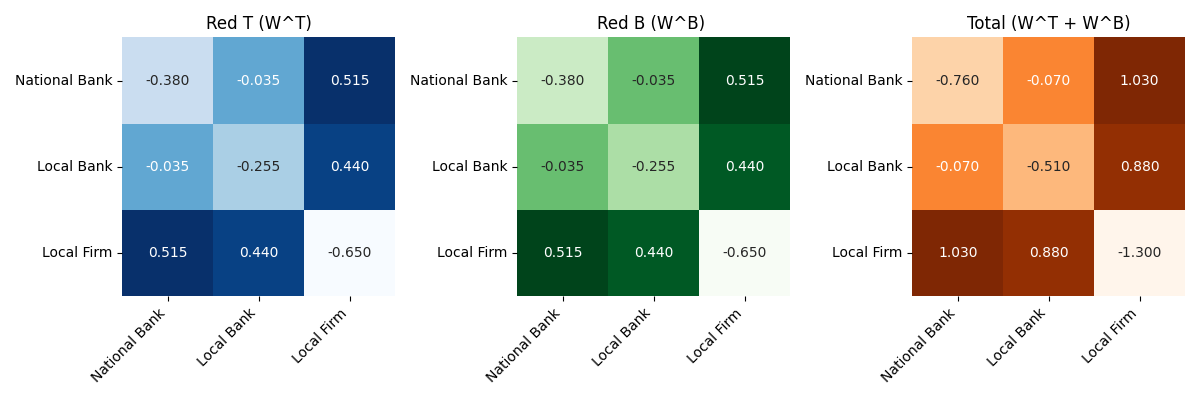
\includegraphics[width=\textwidth,height=0.7\textheight,keepaspectratio]{sin_rest_titulo.png}
  
  \begin{columns}[T]
    \begin{column}{0.55\textwidth}
      \textbf{No Restrictions Case}
      \begin{itemize}
        \item No constraints ($\Psi_i^T = \Psi_i^B = I$)
        \item No transparency benefit ($\tau = 0$)
        \item No blockchain friction ($\lambda_B = 0$)
      \end{itemize}
    \end{column}
    \begin{column}{0.45\textwidth}
      \begin{table}[h]
        \centering
        \begin{tabular}{|l|c|}
          \hline
          Traditional Volume  & 3.265 \\
          \hline
          Blockchain Volume   & 3.265 \\
          \hline
          Total Volume       & 6.530 \\
          \hline
          Blockchain Adoption & 50\% \\
          \hline
        \end{tabular}
      \end{table}
    \end{column}
  \end{columns}
\end{frame}



\begin{frame}{Replication With Two Networks: With Regulatory Constraints}
  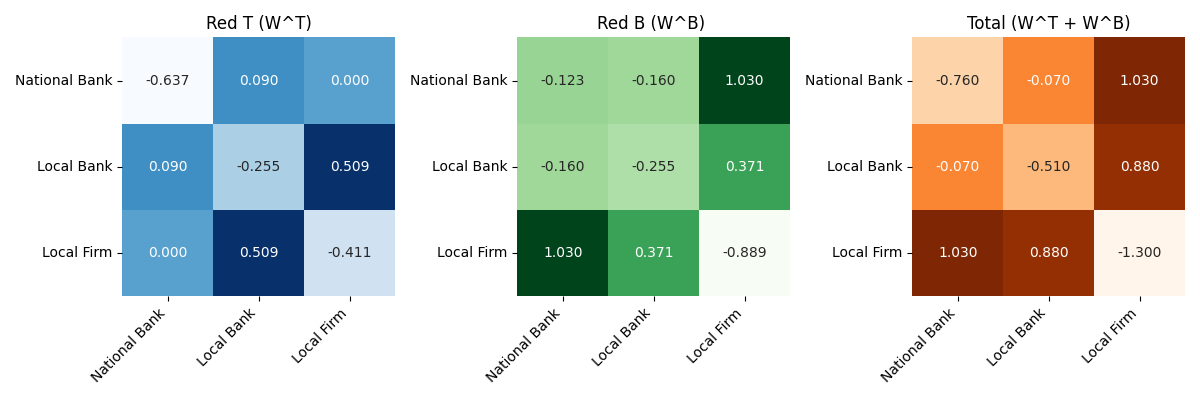
\includegraphics[width=\textwidth,height=0.7\textheight,keepaspectratio]{con_rest_titulo.png}
  
  \begin{columns}[T]
    \begin{column}{0.55\textwidth}
      \textbf{With Restrictions}
      \begin{itemize}
        \item Constraint: Local Bank ↔ Local Firm prohibited in traditional network
        \item No transparency benefit ($\tau = 0$)
        \item No blockchain friction ($\lambda_B = 0$)
      \end{itemize}
    \end{column}
    \begin{column}{0.45\textwidth}
      \begin{table}[h]
        \centering
        \begin{tabular}{|l|c|}
          \hline
          Traditional Volume  & 2.500 \\
          \hline
          Blockchain Volume   & 4.388 \\
          \hline
          Total Volume       & 6.888 \\
          \hline
          Blockchain Adoption & 63.7\% \\
          \hline
        \end{tabular}
      \end{table}
    \end{column}
  \end{columns}
\end{frame}

\begin{frame}{Parameter Effects: $\tau$ and $\lambda_B$}
  \begin{figure}
    \centering
    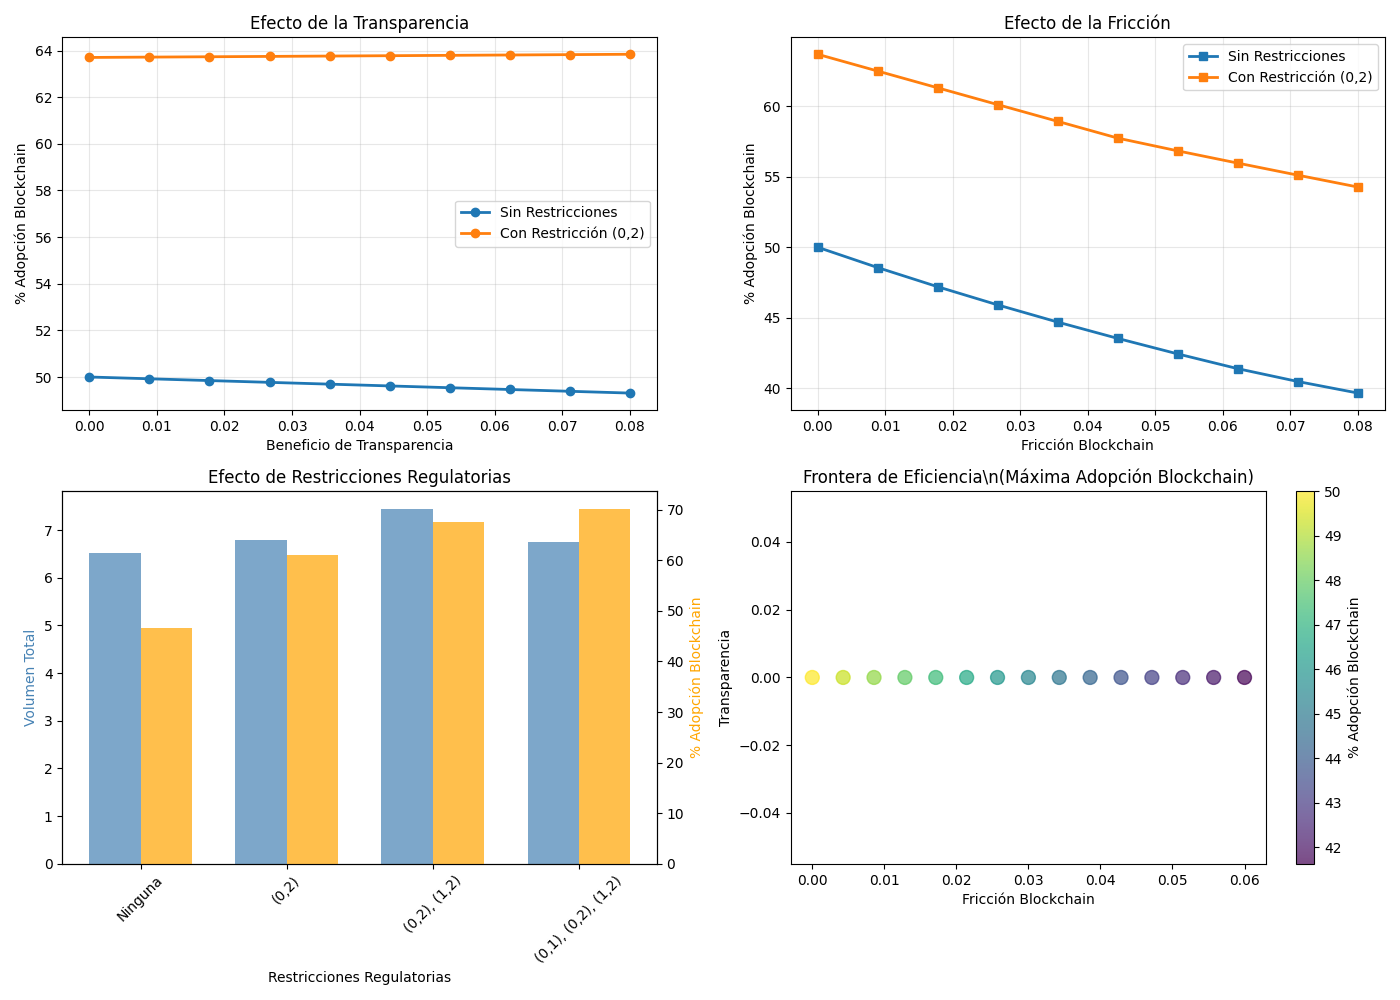
\includegraphics[width=0.95\textwidth]{ex5tauylambda.png}
    \caption{Effects of transparency ($\tau$) and friction ($\lambda_B$) on blockchain adoption}
  \end{figure}
\end{frame}

\begin{frame}{Key Findings Summary}
\textbf{Monte Carlo simulations (2000 iterations):}

\vspace{0.3cm}
\begin{itemize}
    \item \textbf{Baseline adoption:} 50.00\% (symmetric case)
    \item \textbf{Transparency effect} ($\tau=0.1$): \textcolor{blue}{+1.53 pp}
    \item \textbf{Friction effect} ($\lambda_B=0.1$): \textcolor{red}{-12.13 pp}
    \item \textbf{Regulatory constraints:} \textcolor{blue}{+5.35 pp}
\end{itemize}

\vspace{0.3cm}
\textbf{Statistical significance:}
\begin{itemize}
    \item All effects statistically significant (p < 0.001)
    \item Friction has largest impact on adoption
    \item Regulatory constraints favor blockchain adoption
\end{itemize}
\end{frame}

\begin{frame}{Statistical Results}
  \begin{columns}[T]
    \begin{column}{0.32\textwidth}
      \centering
      \textcolor{blue}{\textbf{TRANSPARENCY EFFECT}}
      
      \vspace{0.5em}
      
      \begin{itemize}
        \item H0: $\tau$ has no positive effect
        \item p-value: 0.000001
      \end{itemize}
      
      \vspace{1em}
      
      Transparency has \textbf{positive effect} on blockchain adoption.
    \end{column}
    
    \begin{column}{0.32\textwidth}
      \centering
      \textcolor{blue}{\textbf{FRICTION EFFECT}}
      
      \vspace{0.5em}
      
      \begin{itemize}
        \item H0: $\lambda_B$ does not reduce adoption
        \item p-value: 0.000000
      \end{itemize}
      
      \vspace{1em}
      
      Friction has \textbf{strong negative effect} on blockchain adoption.
    \end{column}
    
    \begin{column}{0.35\textwidth}
      \centering
      \textcolor{blue}{\textbf{REGULATORY EFFECT}}
      
      \vspace{0.5em}
      
      \begin{itemize}
        \item H0: Constraints don't increase blockchain adoption
        \item p-value: 0.000029
      \end{itemize}
      
      \vspace{1em}
      
      Regulatory constraints have \textbf{positive effect} on blockchain adoption.
    \end{column}
  \end{columns}
\end{frame}

\begin{frame}{Detailed Parameter Effects}
  \begin{columns}[T]
    \begin{column}{0.48\textwidth}
      \centering
      \textbf{Friction Effects ($\tau$=0)}
      
      \vspace{0.3em}
      \small{Baseline ($\lambda_B$=0, $\tau$=0): 50.00\%}
      
      \vspace{0.5em}
      
      \begin{table}[h]
        \centering
        \begin{tabular}{|c|c|c|}
          \hline
          \textbf{$\lambda_B$} & \textbf{Adoption} & \textbf{Change} \\
          \hline
          0.0 & 50.00\% & +0.00 pp \\
          \hline
          0.02 & 44.66\% & -5.34 pp \\
          \hline
          0.1 & 37.87\% & -12.13 pp \\
          \hline
          0.2 & 35.83\% & -14.17 pp \\
          \hline
          0.5 & 29.83\% & -20.17 pp \\
          \hline
        \end{tabular}
      \end{table}
    \end{column}
    
    \begin{column}{0.5\textwidth}
      \centering
      \textbf{Transparency Effects ($\lambda_B$=0)}
      
      \vspace{0.3em}
      \small{Baseline ($\lambda_B$=0, $\tau$=0): 50.00\%}
      
      \vspace{0.5em}
      
      \begin{table}[h]
        \centering
        \begin{tabular}{|c|c|c|}
          \hline
          \textbf{$\tau$} & \textbf{Adoption} & \textbf{Change} \\
          \hline
          0.0 & 50.00\% & +0.00 pp \\
          \hline
          0.02 & 51.32\% & +1.32 pp \\
          \hline
          0.1 & 51.53\% & +1.53 pp \\
          \hline
          0.2 & 51.70\% & +1.70 pp \\
          \hline
          0.5 & 53.41\% & +3.41 pp \\
          \hline
        \end{tabular}
      \end{table}
    \end{column}
  \end{columns}
\end{frame}

\begin{frame}{Visual Results}
  \begin{columns}[T]
    \begin{column}{0.55\textwidth}
      \centering
      \textbf{Friction Impact}
      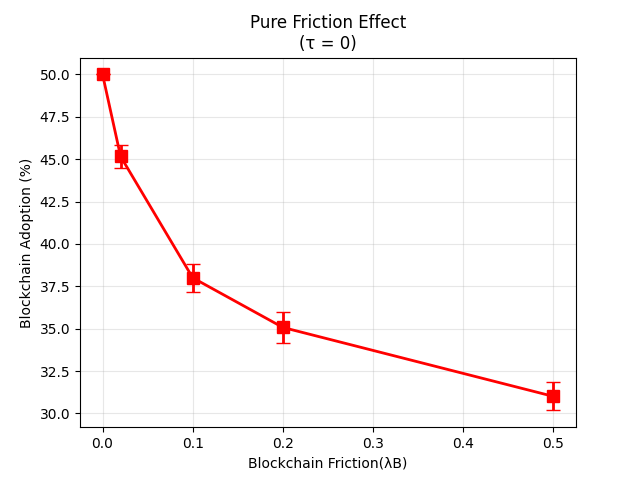
\includegraphics[width=\textwidth]{friction.png}
    \end{column}
    \begin{column}{0.55\textwidth}
      \centering
      \textbf{Transparency Impact}
      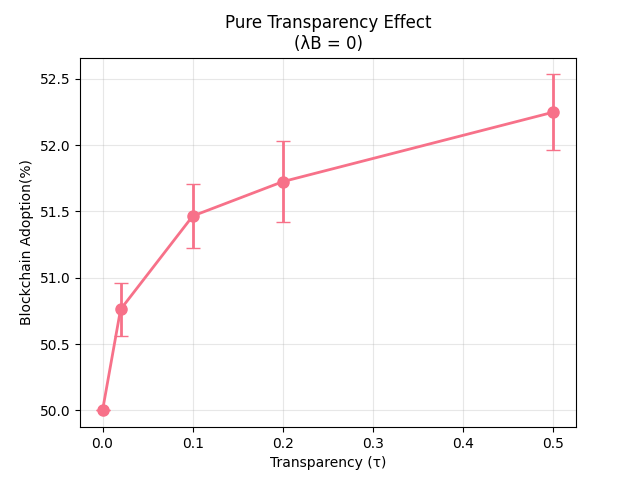
\includegraphics[width=\textwidth]{transp.png}
    \end{column}
  \end{columns}
\end{frame}

\begin{frame}{Current Work and Next Steps}
\textbf{Ongoing research:}
\begin{itemize}
\item \textbf{Mathematical verification:}
    \begin{itemize}
        \item Algebraic consistency between theoretical derivations and simulations
        \item Validation of convergence properties and theorems
    \end{itemize}
    
\item \textbf{Parameter calibration:}
    \begin{itemize}
        \item Empirical estimation of transparency benefit $\tau$
        \item Calibration of friction parameter $\lambda_B$ using real data
    \end{itemize}
    
\item \textbf{Model applications:}
    \begin{itemize}
        \item Extension to donation and charity networks
        \item Cross-border payment systems analysis
    \end{itemize}
\end{itemize}
\end{frame}

\begin{frame}{Conclusions and Policy Implications}
\textbf{Main findings:}
\begin{itemize}
    \item \textcolor{blue}{Transparency has positive but modest effects} on blockchain adoption (+1.53 pp)
    \item \textcolor{red}{Friction has strong negative effects} on adoption (-12.13 pp)
    \item \textcolor{blue}{Regulatory constraints favor blockchain} adoption (+5.35 pp)
    \item Network effects amplify individual agent decisions
\end{itemize}




\end{frame}



\begin{frame}{Current Work}
\begin{itemize}
\item Algebraic review of numerical results
    \begin{itemize}
        \item Mathematical verification of consistency between theoretical derivations and simulations.
        \item Validation of convergence properties and theorems.
    \end{itemize}
\item Calibration of new parameters.
    \begin{itemize}
        \item Empirical estimation of $\tau$.
        \item Calibration of $\lambda$.
    \end{itemize}
\item Model adjustment to donation data.
\end{itemize}
\end{frame}

\begin{frame}[allowframebreaks]{References}
\begin{thebibliography}{9}
\bibitem{pwc2020}
PwC. (2020). 
\textit{Blockchain could boost the global economy by \$1.76 trillion by 2030 through raising levels of tracking, tracing and trust}. 
Available at: \url{https://www.pwc.com/gx/en/news-room/press-releases/2020/blockchain-boost-global-economy-track-trace-trust.html}

\bibitem{jalan2024}
Jalan, A., Chakrabarti, D., \& Sarkar, P. (2024). 
\textit{Incentive-Aware Models of Financial Networks}. 
Operations Research, Articles in Advance.

\bibitem{market_research_future2024}
Market Research Future. (2024). 
\textit{Global Blockchain FinTech Market Research Report}.
\end{thebibliography}
\end{frame}
\end{document}